\definecolor{cOne}{HTML}{4C78A8}
\definecolor{cTwo}{HTML}{F58518}
\definecolor{cThree}{HTML}{54A24B}
\definecolor{cFour}{HTML}{8E6BBE}
\definecolor{cFive}{HTML}{E45756}
\definecolor{tfgrey}{HTML}{9CA3AF}
\definecolor{tfsoft}{HTML}{F3F4F6}

\newcommand{\wedgeobs}[6]{%
  % #1 x, #2 y, #3 scale, #4 label, #5 swapped flag, #6 subtitle
  \begin{scope}[shift={(#1,#2)}, scale=#3]
    \draw[black, line width=0.6pt] (0,0) circle (0.82);
    \ifnum#5=0
      \fill[cTwo!35]   (0,0) -- (90:0.82) -- (0:0.82) -- cycle;
      \fill[cFour!35]  (0,0) -- (0:0.82) -- (-90:0.82) -- cycle;
      \fill[cOne!35]   (0,0) -- (-90:0.82) -- (180:0.82) -- cycle;
      \fill[cThree!35] (0,0) -- (180:0.82) -- (90:0.82) -- cycle;

      \node[text=cTwo,   font=\scriptsize] at (45:0.43) {$c_2$};
      \node[text=cFour,  font=\scriptsize] at (-45:0.43) {$c_4$};
      \node[text=cOne,   font=\scriptsize] at (-135:0.43) {$c_1$};
      \node[text=cThree, font=\scriptsize] at (135:0.43) {$c_3$};
    \else
      \fill[cTwo!35]   (0,0) -- (90:0.82) -- (0:0.82) -- cycle;
      \fill[cOne!35]   (0,0) -- (0:0.82) -- (-90:0.82) -- cycle;
      \fill[cFour!35]  (0,0) -- (-90:0.82) -- (180:0.82) -- cycle;
      \fill[cThree!35] (0,0) -- (180:0.82) -- (90:0.82) -- cycle;

      \node[text=cTwo,   font=\scriptsize] at (45:0.43) {$c_2$};
      \node[text=cOne,   font=\scriptsize] at (-45:0.43) {$c_1$};
      \node[text=cFour,  font=\scriptsize] at (-135:0.43) {$c_4$};
      \node[text=cThree, font=\scriptsize] at (135:0.43) {$c_3$};
    \fi

    \draw[black, line width=0.6pt] (0,0) -- (90:0.82);
    \draw[black, line width=0.6pt] (0,0) -- (0:0.82);
    \draw[black, line width=0.6pt] (0,0) -- (-90:0.82);
    \draw[black, line width=0.6pt] (0,0) -- (180:0.82);
    \fill[black] (0,0) circle (0.045);

    \node[font=\footnotesize] at (0,-1.12) {#4};
    \node[font=\scriptsize\itshape, align=center, text=tfgrey] at (0,-1.45) {#6};
  \end{scope}
}

\resizebox{\columnwidth}{!}{%
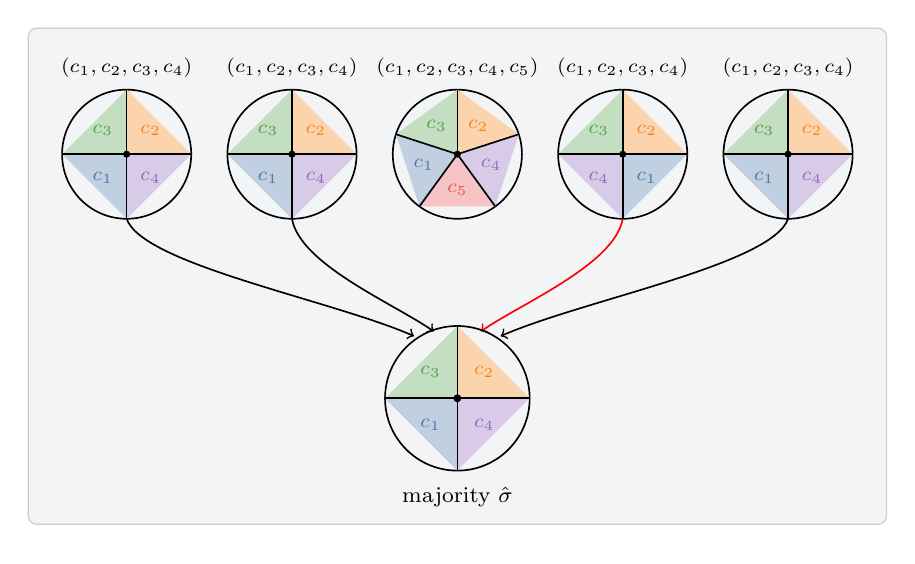
\begin{tikzpicture}[font=\rmfamily\footnotesize]

  % Panel background.
  \filldraw[fill=tfsoft, draw=black!20, line width=0.4pt, rounded corners=3pt]
    (-5.45,-2.75) rectangle (5.45,3.55);

  % Top row: four observations of equivalence class (c_1, c_2, c_3, c_4).
  \wedgeobs{-4.20}{1.95}{1.0}{}{0}{}
  \wedgeobs{-2.10}{1.95}{1.0}{}{0}{}
  \wedgeobs{ 2.10}{1.95}{1.0}{}{1}{}
  \wedgeobs{ 4.20}{1.95}{1.0}{}{0}{}

  \node[font=\scriptsize] at (-4.20,3.05) {$(c_1, c_2, c_3, c_4)$};
  \node[font=\scriptsize] at (-2.10,3.05) {$(c_1, c_2, c_3, c_4)$};
  \node[font=\scriptsize] at ( 2.10,3.05) {$(c_1, c_2, c_3, c_4)$};
  \node[font=\scriptsize] at ( 4.20,3.05) {$(c_1, c_2, c_3, c_4)$};

  % Middle wedge: different equivalence class with 5 components.
  % Permutation = majority (c_2, c_4, c_1, c_3) with c_5 inserted between c_4 and c_1.
  \begin{scope}[shift={(0,1.95)}, scale=1.0]
    \draw[black, line width=0.6pt] (0,0) circle (0.82);
    \fill[cTwo!35]   (0,0) -- (90:0.82)   -- (18:0.82)   -- cycle;
    \fill[cFour!35]  (0,0) -- (18:0.82)   -- (-54:0.82)  -- cycle;
    \fill[cFive!35]  (0,0) -- (-54:0.82)  -- (-126:0.82) -- cycle;
    \fill[cOne!35]   (0,0) -- (-126:0.82) -- (162:0.82)  -- cycle;
    \fill[cThree!35] (0,0) -- (162:0.82)  -- (90:0.82)   -- cycle;

    \node[text=cTwo,   font=\scriptsize] at (54:0.45)   {$c_2$};
    \node[text=cFour,  font=\scriptsize] at (-18:0.45)  {$c_4$};
    \node[text=cFive,  font=\scriptsize] at (-90:0.45)  {$c_5$};
    \node[text=cOne,   font=\scriptsize] at (-162:0.45) {$c_1$};
    \node[text=cThree, font=\scriptsize] at (126:0.45)  {$c_3$};

    \draw[black, line width=0.6pt] (0,0) -- (90:0.82);
    \draw[black, line width=0.6pt] (0,0) -- (18:0.82);
    \draw[black, line width=0.6pt] (0,0) -- (-54:0.82);
    \draw[black, line width=0.6pt] (0,0) -- (-126:0.82);
    \draw[black, line width=0.6pt] (0,0) -- (162:0.82);
    \fill[black] (0,0) circle (0.045);
  \end{scope}

  \node[font=\scriptsize] at (0,3.05) {$(c_1, c_2, c_3, c_4, c_5)$};

  % Vote convergence arrows.
  \draw[->, line width=0.6pt, black]
    (-4.20,1.13) .. controls (-4.00,0.55) and (-1.60,0.10) .. (-0.55,-0.36);
  \draw[->, line width=0.6pt, black]
    (-2.10,1.13) .. controls (-2.00,0.55) and (-0.80,0.05) .. (-0.30,-0.30);
  \draw[->, line width=0.6pt, red]
    ( 2.10,1.13) .. controls ( 2.00,0.55) and ( 0.80,0.05) .. ( 0.30,-0.30);
  \draw[->, line width=0.6pt, black]
    ( 4.20,1.13) .. controls ( 4.00,0.55) and ( 1.60,0.10) .. ( 0.55,-0.36);

  \wedgeobs{0}{-1.15}{1.12}{majority $\hat{\sigma}$}{0}{}

\end{tikzpicture}%
}
